\documentclass[9pt,twocolumn,twoside]{pnas-report}

\templatetype{pnasresearcharticle}

\usepackage{lipsum}
\usepackage{subcaption}

\title{Chess Network: A Hybrid Absorbing Markov Chain and Pathfinding Approach}

\author[a]{Luka Bajić}
\author[a]{Matej Belšak}
\author[b]{Vanja Stojanović}

\affil[a]{University of Ljubljana, Faculty of Computer and Information Science, Ve\v{c}na pot 113, SI-1000 Ljubljana, Slovenia}
\affil[b]{University of Ljubljana, Faculty of Mathematics and Physics, Jadranska cesta 21, SI-1000 Ljubljana, Slovenia}

\leadauthor{Matej Belšak} 
%\authordeclaration{All authors contributed equally to this work.}
%\correspondingauthor{\textsuperscript{1}To whom correspondence should be addressed. E-mail: lb4129@student.uni-lj.si}

\begin{abstract}
Modern chess engines evaluate positions in isolation, ignoring the broader network structure of the game. Consequently, seemingly strong positions can be fragile if surrounded by losing states. We propose a novel hybrid heuristic that evaluates entire communities of game states rather than single nodes. We mapped the state space using limited-depth DFS and assigned Win/Draw/Loss states using Syzygy tablebases. We extracted communities using the Leiden algorithm and formalized the macro-network as an Absorbing Markov Chain (AMC) to model global defeat probabilities under perfect opponent play. By converting these risk values into dynamic edge weights, we applied Dijkstra's algorithm to compute globally robust, safe strategic paths. To reduce computational costs, we tested sampling methods. Results show probabilistic DFS sampling is highly practical, maintaining strong community structure (NMI of 0.898 at a 0.8 probability for depth 7). This scalable framework effectively guides engines through structurally safe regions of the game space.
\end{abstract}

%\dates{The manuscript was compiled on \today}
\doi{\href{https://ucilnica.fri.uni-lj.si/course/view.php?id=183}{Introduction to Network Analysis} 2025/26}

\begin{document}

\maketitle
\thispagestyle{firststyle}
\ifthenelse{\boolean{shortarticle}}{\ifthenelse{\boolean{singlecolumn}}{\abscontentformatted}{\abscontent}}{}

\dropcap{S}{\bf tate-of-the-art chess engines use techniques} such as Monte Carlo Tree Search \cite{mcts} and alpha-beta pruning \cite{alphabeta} for search and deep neural networks to evaluate positions and look for an optimal playing strategy. However, they do not consider the network structure of the state space of the game, meaning that the quality of the solution depends entirely on the evaluations of individual positions.

In this work, we propose a network analysis approach to guide the search. Instead of evaluating a position in isolation, we assess the broader community of states to which it belongs. The intuition behind this is that a seemingly good position might be fragile if it is surrounded by losing states. We map the local state space by exploring all legal moves from a starting position up to a limited depth using Depth First Search (DFS). For endgames, we can assign an exact Win, Draw, or Loss (WDL) state to each node using Syzygy tablebases \cite{syzygy}. For general positions WDL can be approximated, so this approach can be generalized - we provide a network generator, as well as all remaining implementation\footnote{https://github.com/matejck/Chess-endgame-network-analysis/tree/main}. We then extract communities using the Leiden algorithm \cite{leiden}. To evaluate the systemic vulnerability of these groups, we model the macro-network as an Absorbing Markov Chain, partitioning communities into transient regions and absorbing zones of imminent defeat or guaranteed victory. By deriving global absorption probabilities, we generate risk-aware edge weights to run Dijkstra's algorithm \cite{dijkstra}. This hybrid method naturally guides the search through safe regions of state space, while heavily penalizing paths passing through dynamically risky or bad communities.

For computational purposes, we also test whether network sampling preserves communities. We use Normalized Mutual Information (NMI) to evaluate how well probabilistic node-induced sampling (Node sampling) and probabilistic DFS edge-induced sampling (DFS sampling) preserve the original community structure. By comparing these techniques across different sampling rates, we investigate the trade-offs between reducing the network size and maintaining structural accuracy.

\section*{Related work}

Typical applications of network analysis techniques in the domain of chess include encoding an individual position on the board \cite{chess} with the goal of predicting the outcome of the game, an analysis tool of the openings with respect to the skill level of the players \cite{chess3}, clustering methods used on the openings to infer the result or other properties of the game \cite{chess2}, and using network-based metrics to quantify interaction between pieces \cite{chess4}. These approaches use either externally gathered data or a network generated from a single chess position. In this paper, we aim to expand this to arbitrarily large networks that can be generated for any starting position. 

\section*{Results}
We generate a state space network from the starting position with EPD: \texttt{3r4/2k5/5P2/7K/8/8/8/8 b - -}. We limit the generation to maximum depths of 5 and 7 to evaluate scalability and visualized the resulting networks using the ForceAtlas2 \cite{atlas} graph layout algorithm, as shown in Figure \ref{fig.network1}.

To identify favorable regions, we ranked communities by individual quality ($\mathcal{Q}_{0.5}$) and calculated the cumulative path cost ($\mathcal{C}_{0.5}$) from the community containing the starting state to all other communities using Dijkstra's algorithm.

To test structural robustness under computational constraints, we averaged NMI over 25 repetitions for both Node sampling and DFS sampling with varying probabilities ($p$).

\subsection{Network with maximum depth of 5}
We first evaluated the state space network bounded to a maximum search depth of 5, yielding a network with $19 ^\cdot 607$ nodes and $75 ^\cdot 160$ edges. The results are shown in Table \ref{table.network1.scores}, Table \ref{table.network1.NMI} and Figure \ref{fig.network1}.

\begin{table}[ht]
\centering
\caption{Comparison of the top 5 communities ranked by individual community quality $\mathcal{Q}_{0.5}^\textnormal{norm}$ and safest reachable targets by path cost ($\mathcal{Q}_{0.5}^\text{norm}$) for depth 5.}
\begin{tabular}{c l l}
\hline
\textbf{Rank} & \textbf{Best $\mathcal{Q}_{0.5}^\textnormal{norm}$ Scores} & \textbf{Lowest Path Cost ($\mathcal{C}_{0.5}$)} \\
\hline
$1$ & $0.938$ (Community 14) & $0.000$ (Community 11) \\
$2$ & $0.897$ (Community 12) & $0.186$ (Community 1) \\
$3$ & $0.891$ (Community 15) & $0.249$ (Community 14) \\
$4$ & $0.831$ (Community 1) & $0.295$ (Community 12) \\
$5$ & $0.820$ (Community 11) & $0.301$ (Community 15) \\
\hline
\end{tabular}
\label{table.network1.scores}
\end{table}

\begin{figure*}[t]
    \centering
    \begin{subfigure}{0.32\linewidth}
        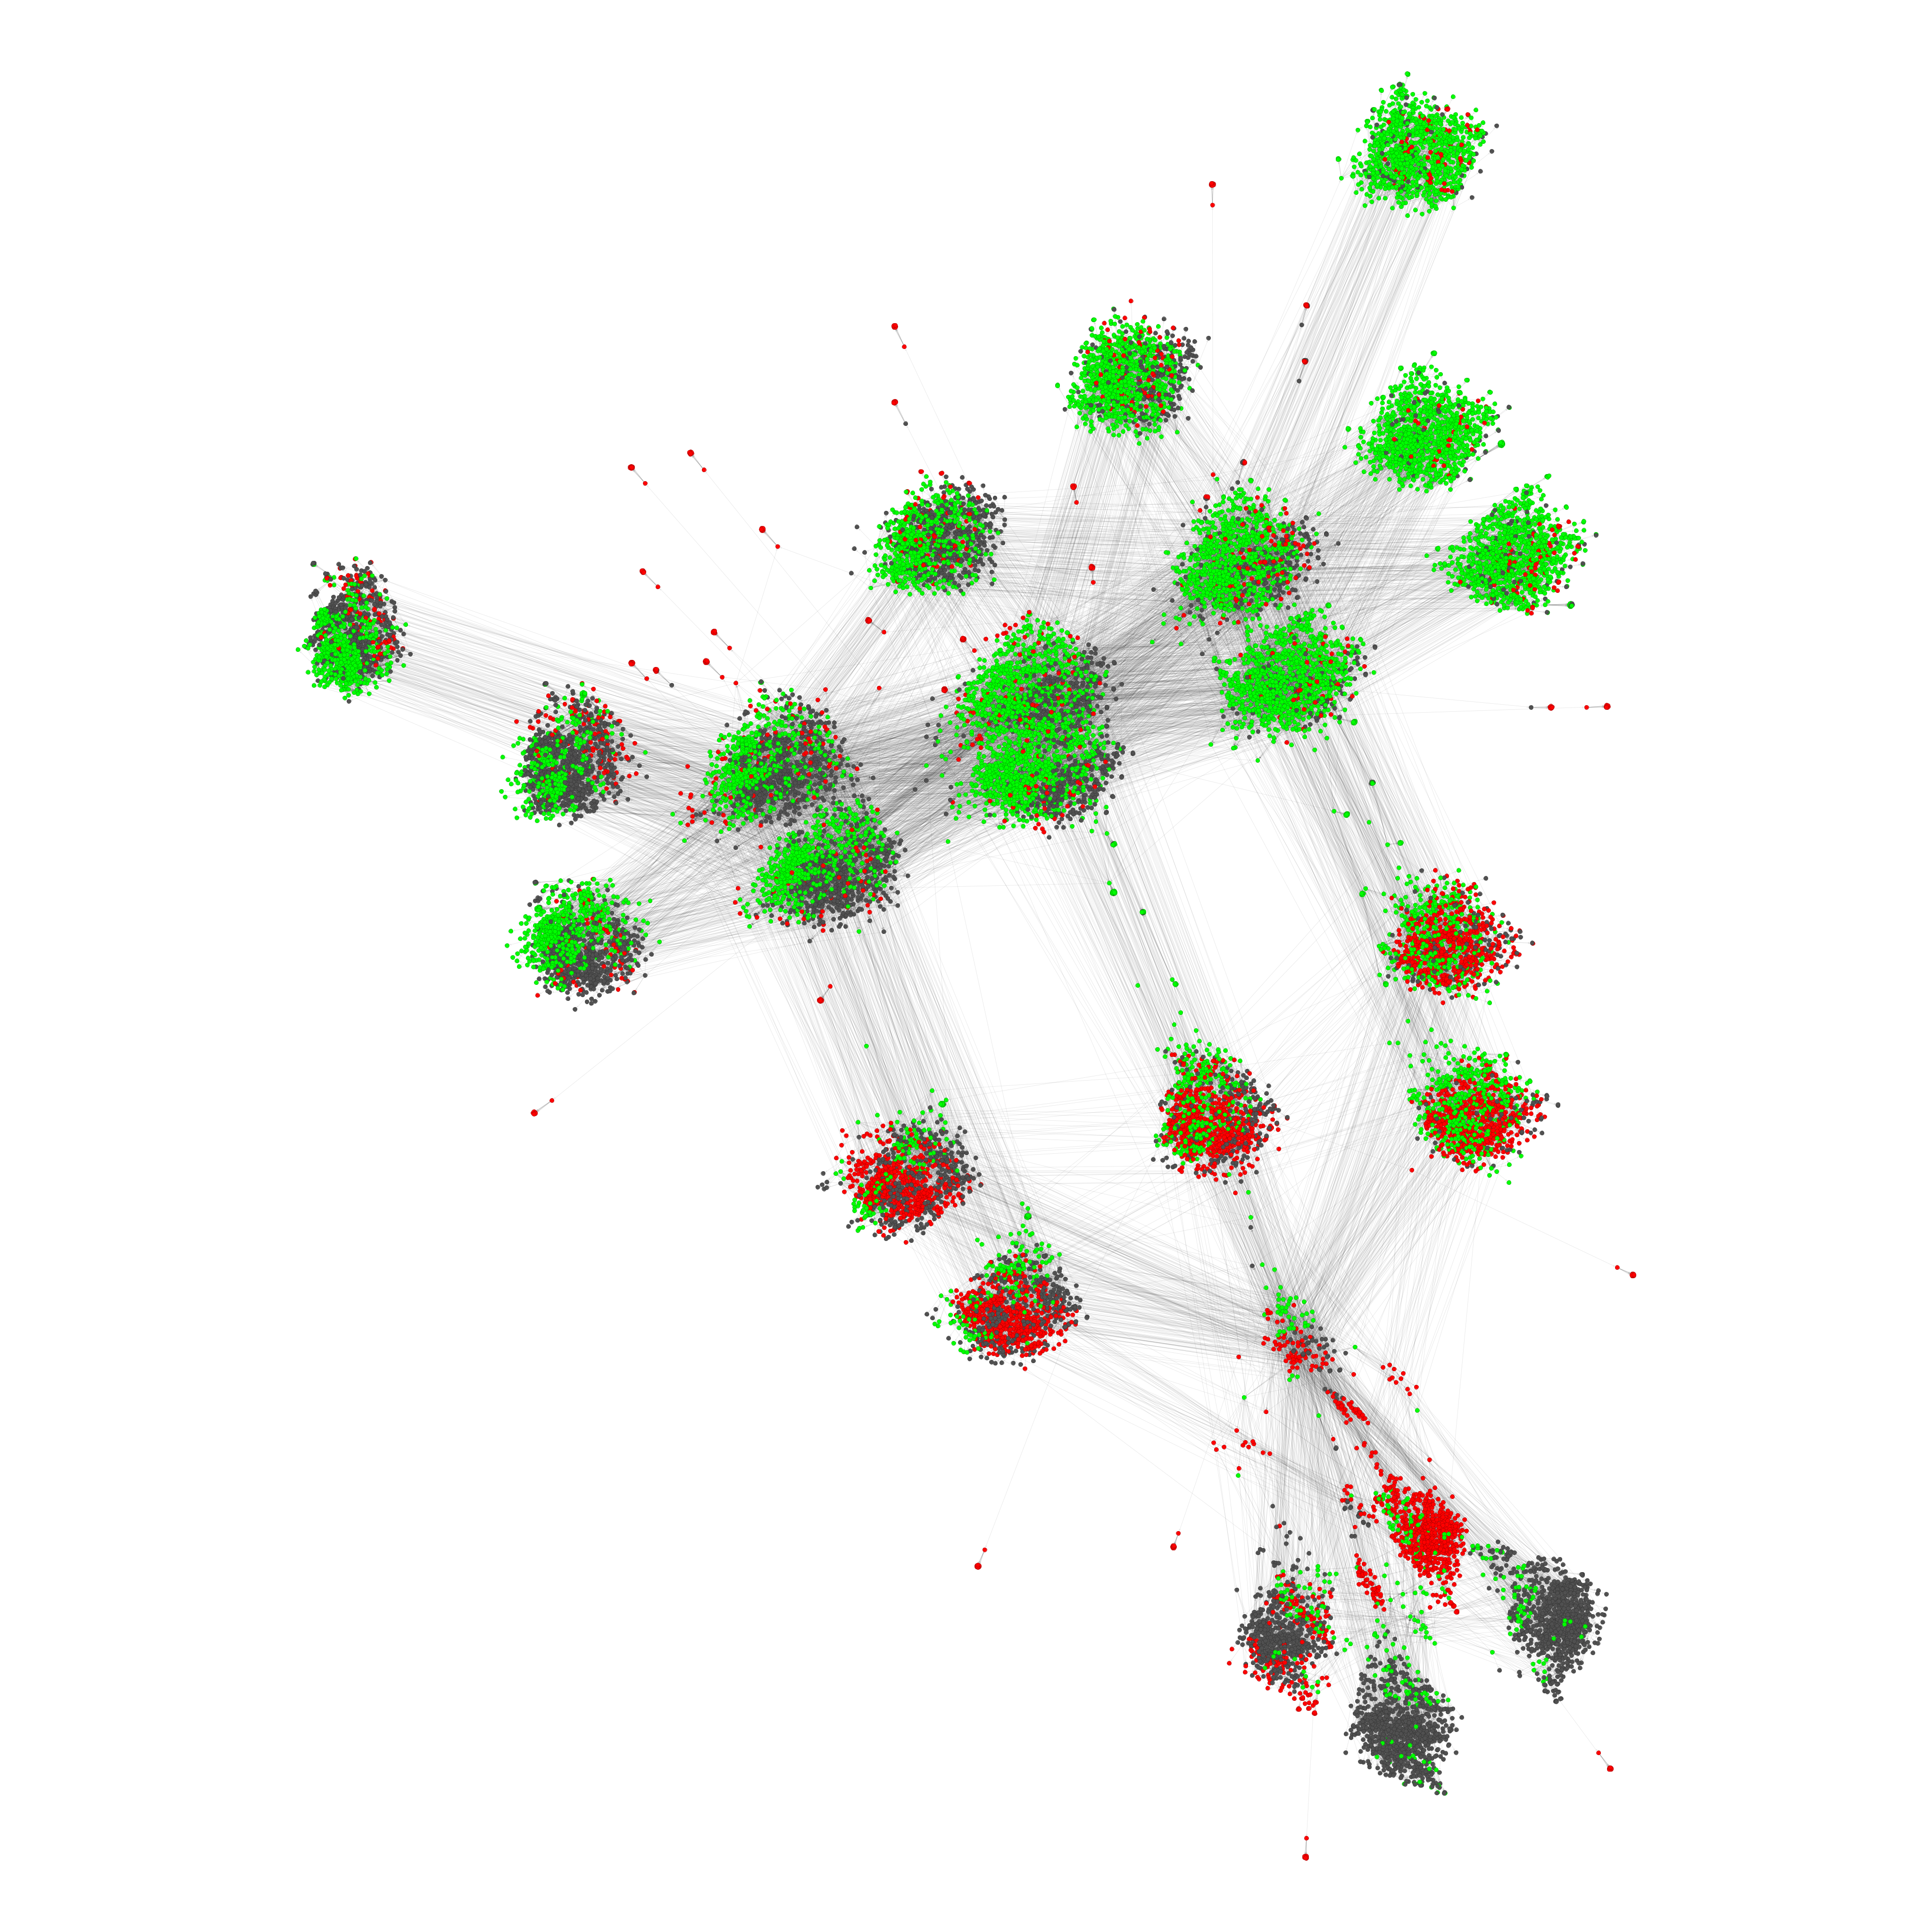
\includegraphics[width=\linewidth, trim={600 256 600 128}, clip]{results/network1/KRvKP_5_wdl.png}
        \centering
        \caption{Original network}
        \label{fig.network1.wdl}
    \end{subfigure}\hfill
    \begin{subfigure}{0.32\linewidth}
        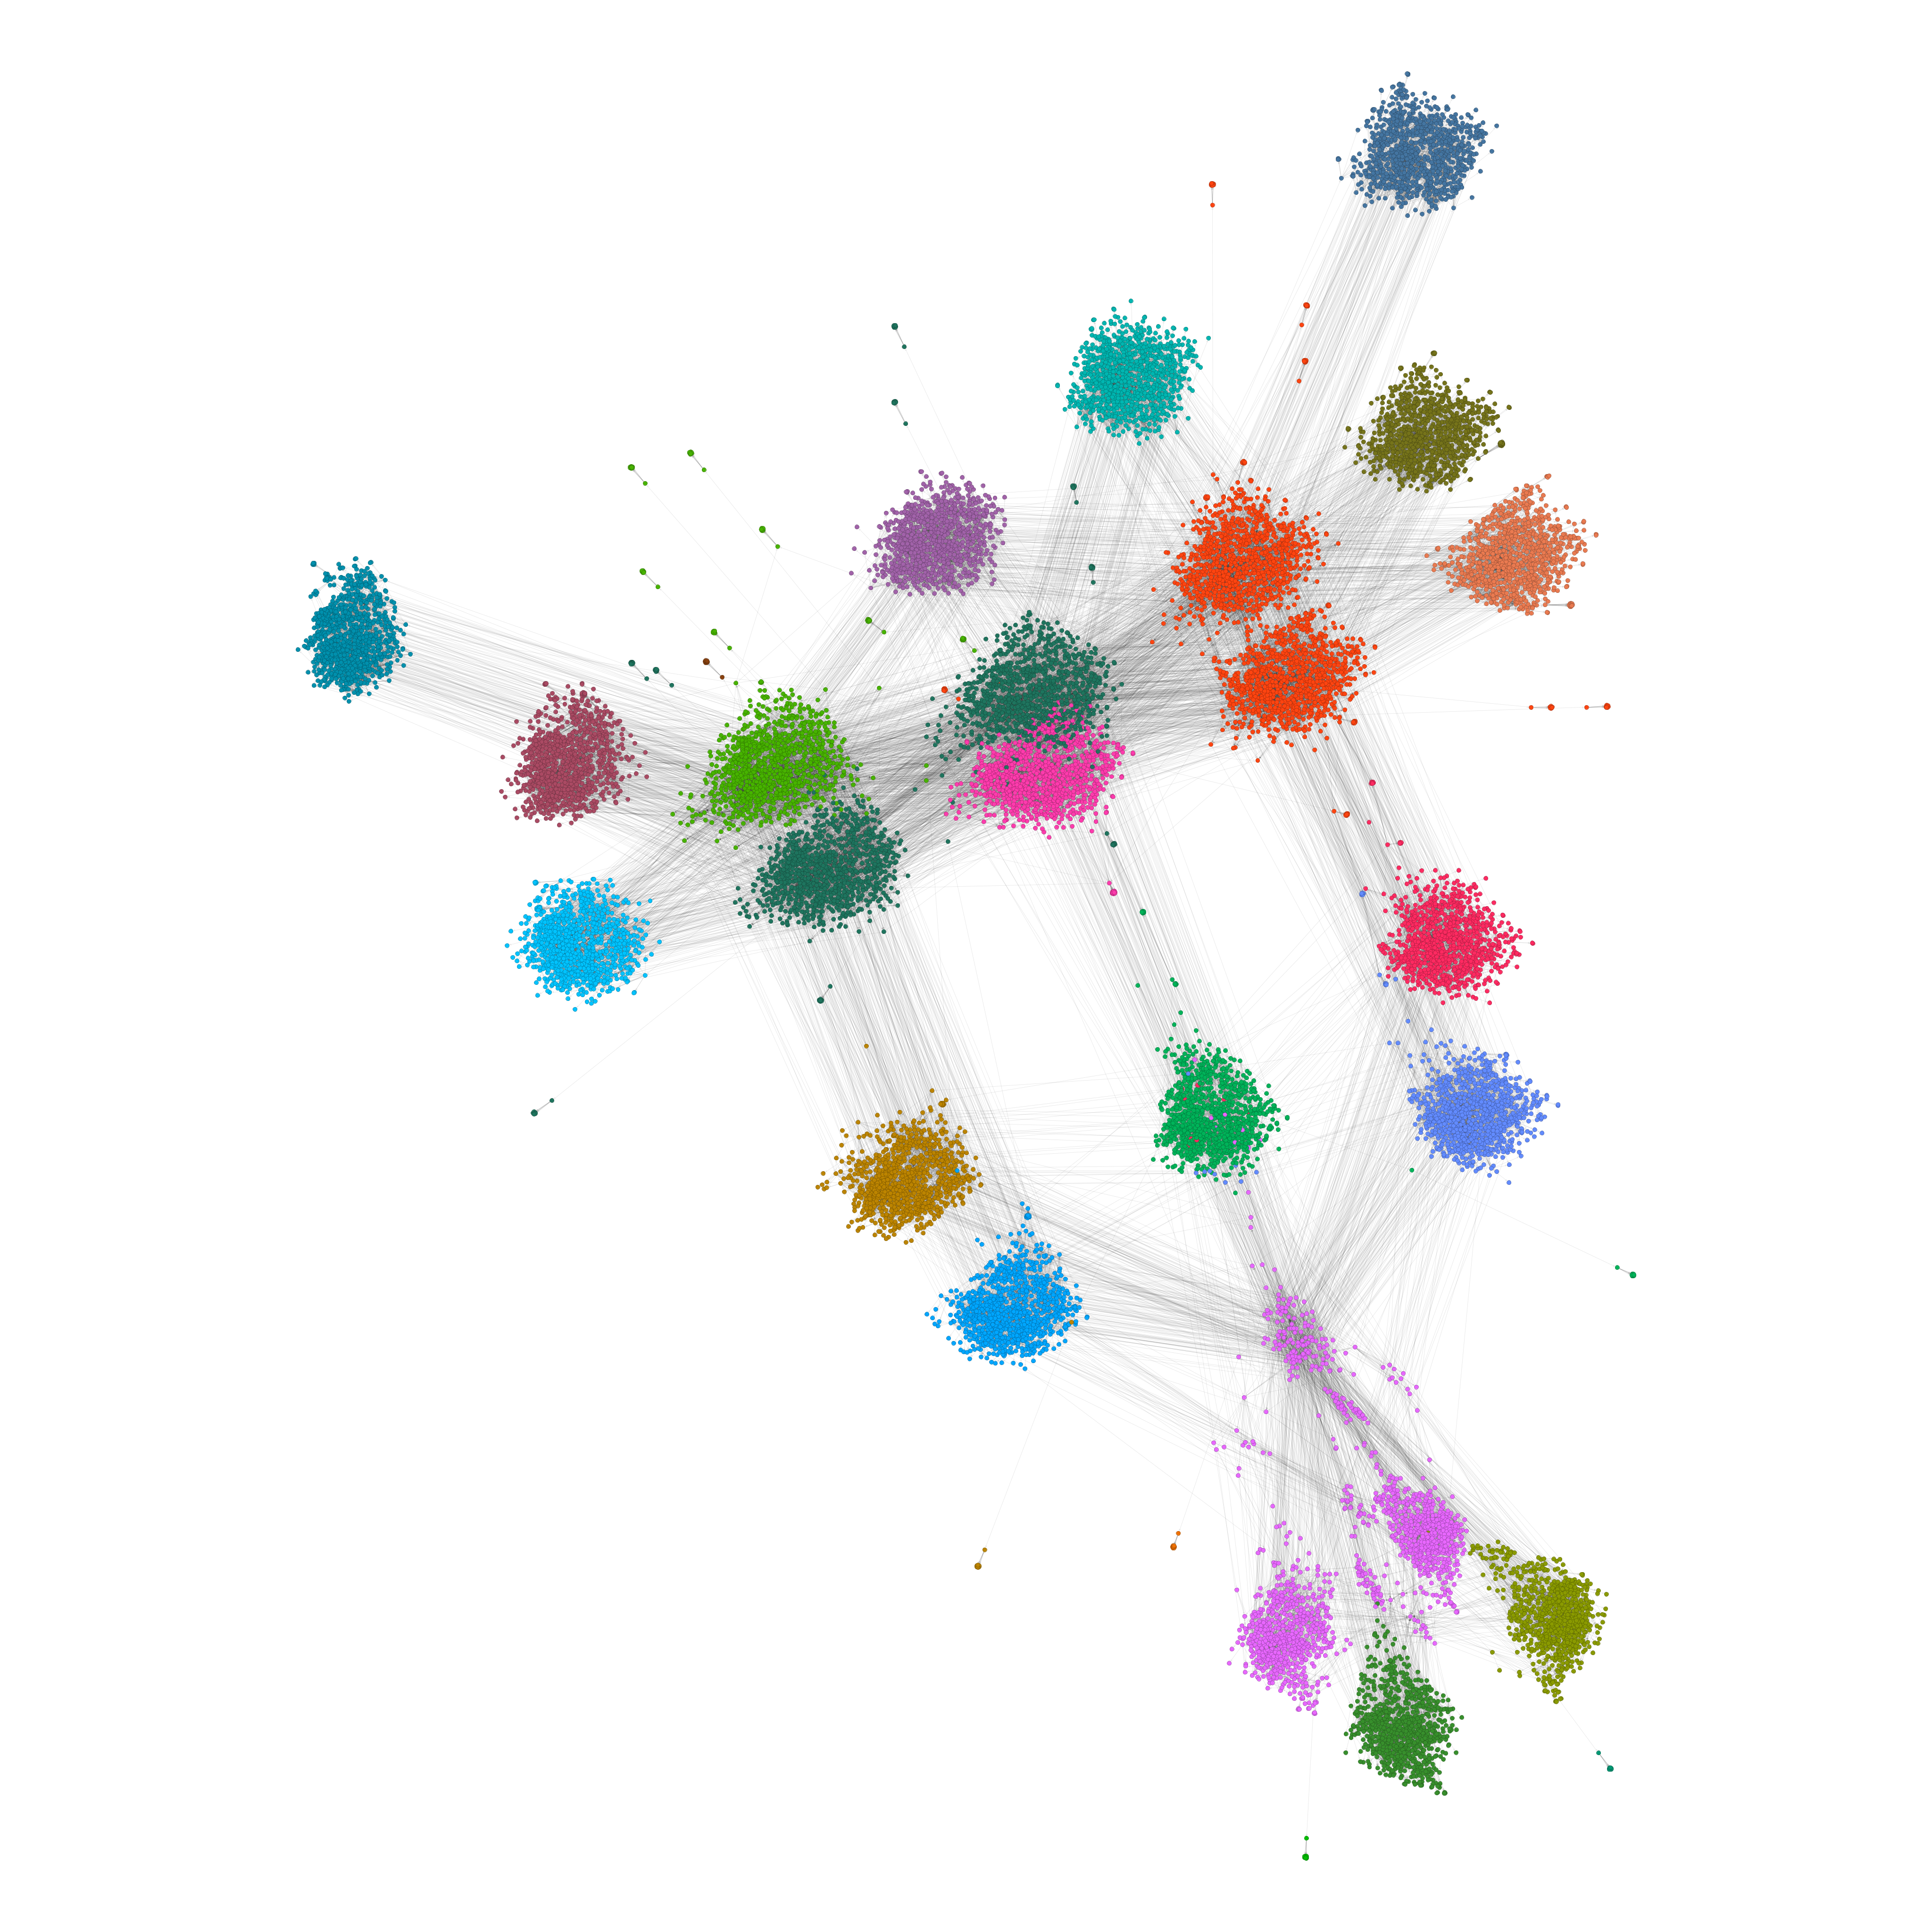
\includegraphics[width=\linewidth, trim={600 256 600 128}, clip]{results/network1/KRvKP_5_leiden.png}
        \centering
        \caption{Original network with communities}
        \label{fig.network1.leiden}
    \end{subfigure}
    \begin{subfigure}{0.32\linewidth}
        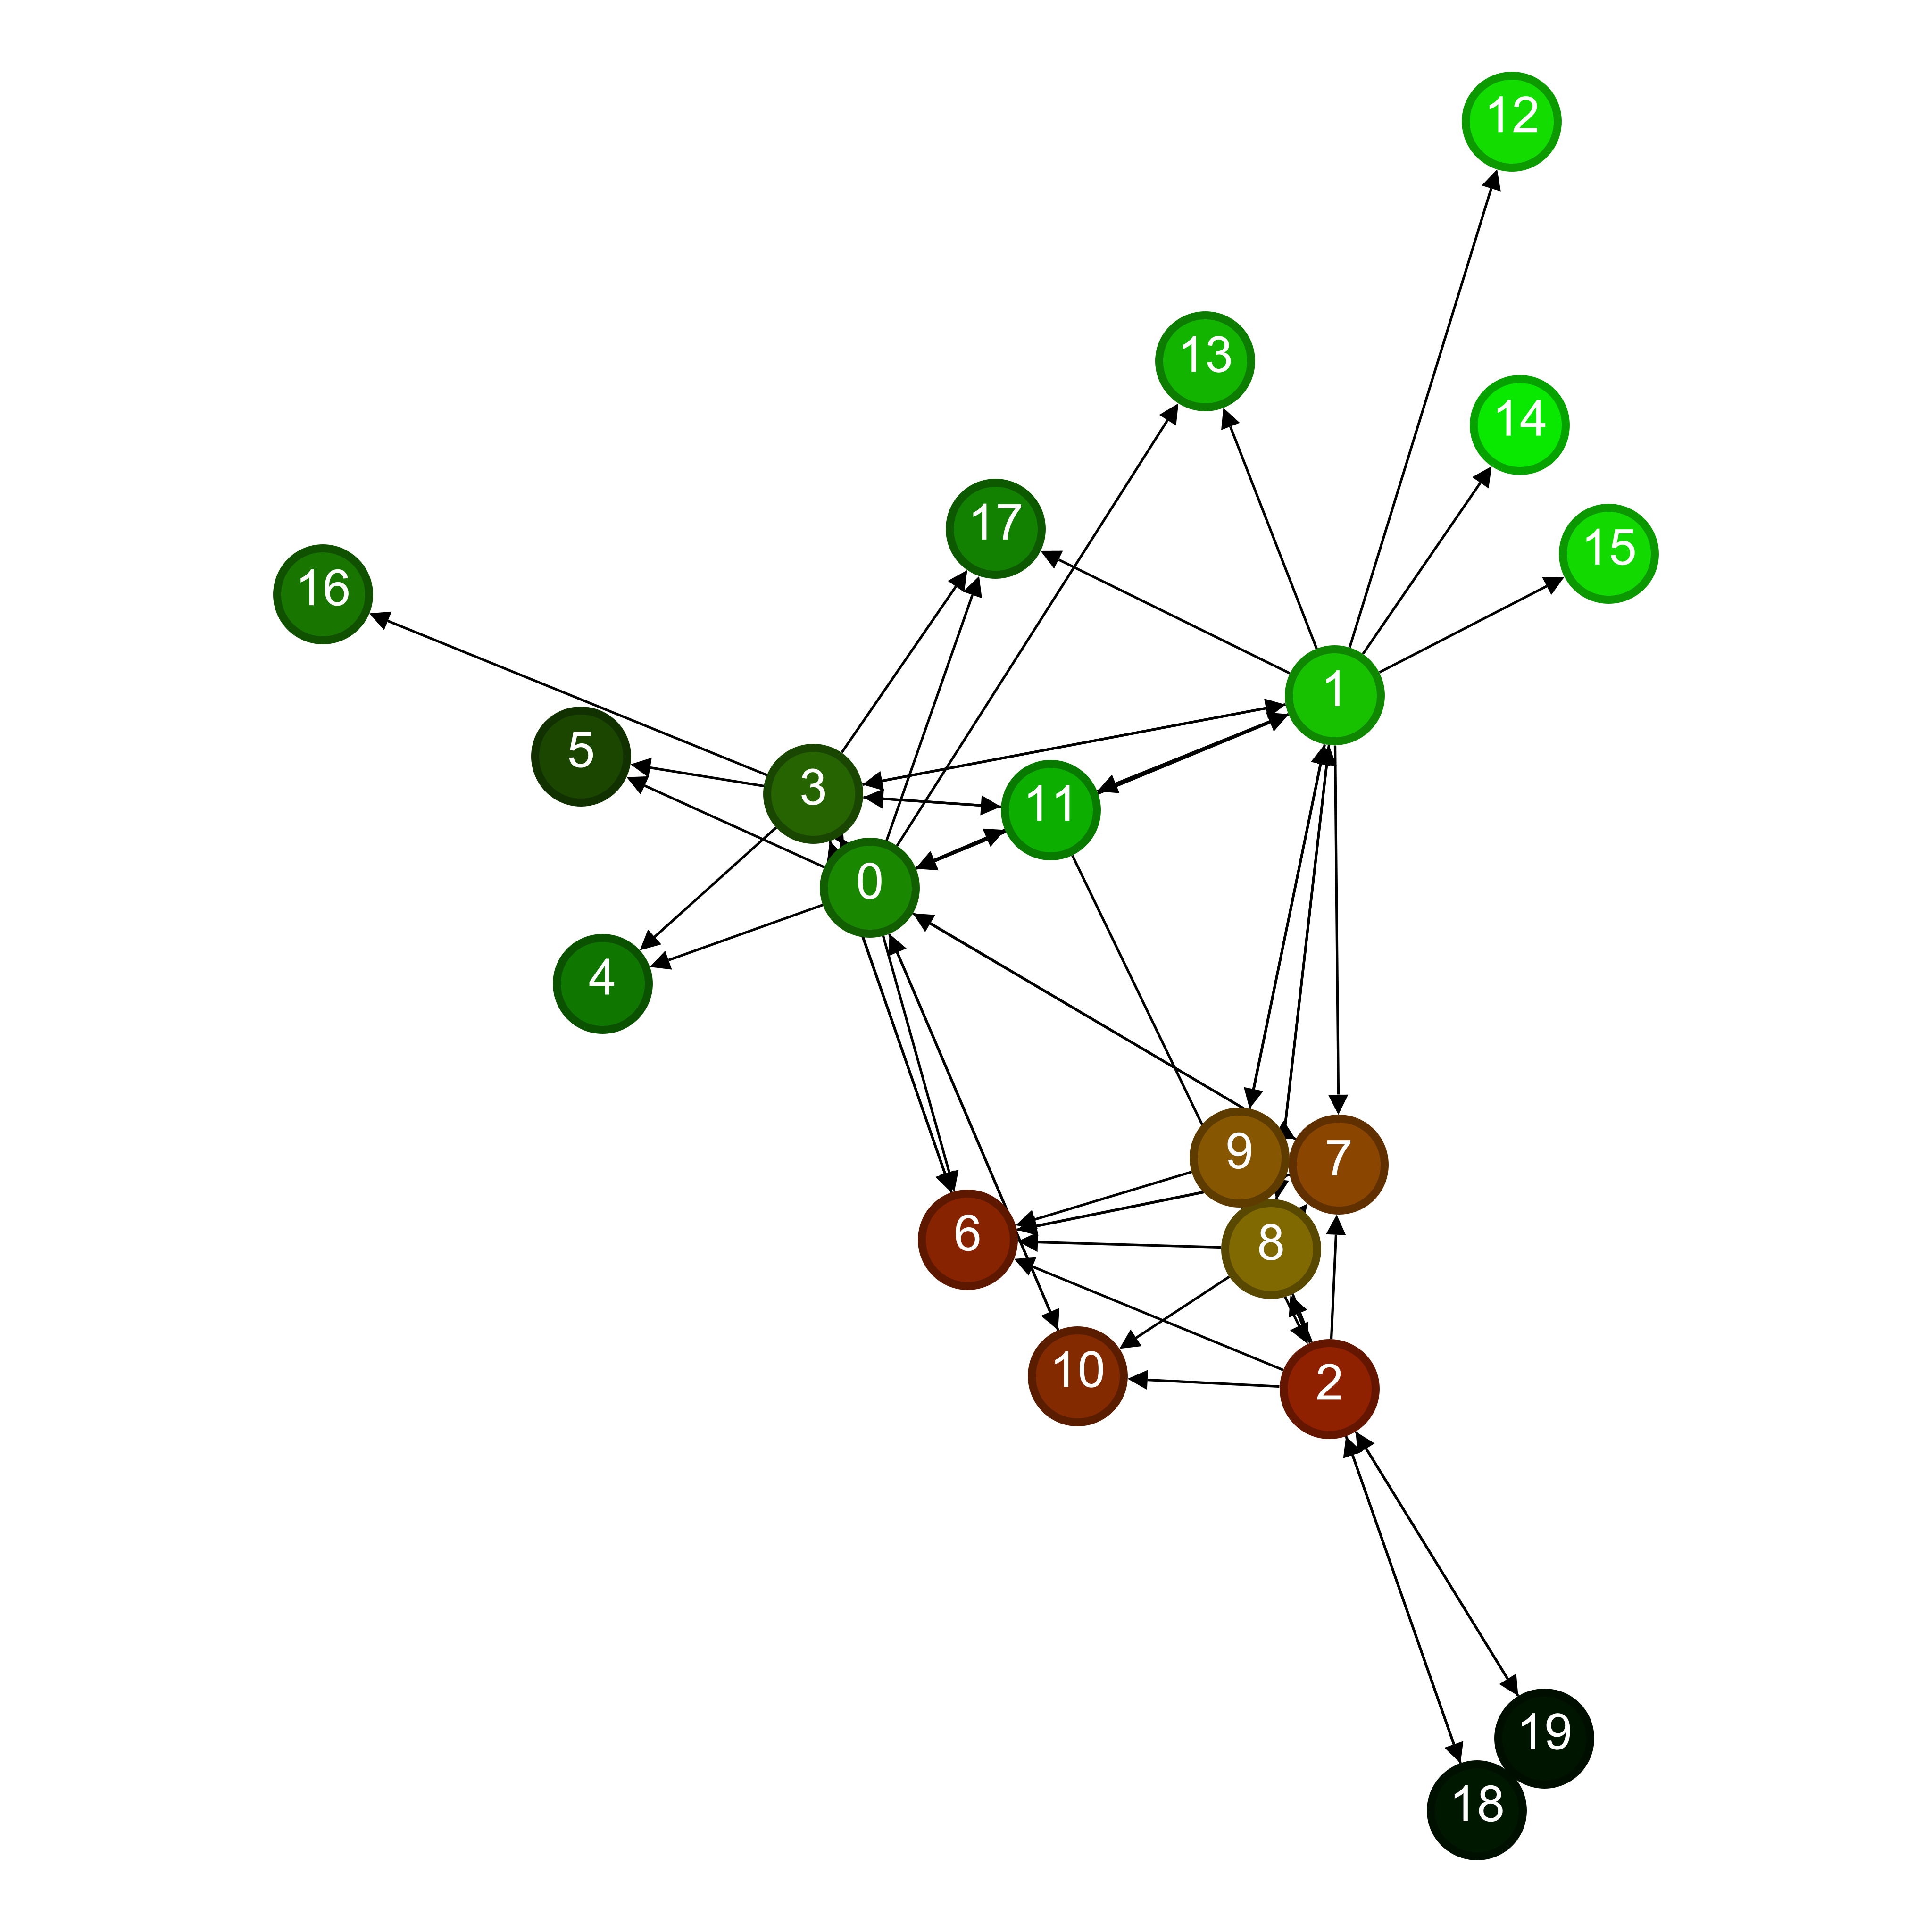
\includegraphics[width=\linewidth, trim={512 128 512 128}, clip]{results/network1/KRvKP_5_community.png}
        \centering
        \caption{Community network}
        \label{fig.network1.community}
    \end{subfigure}
    \caption{Visualizations of the state space. Graph \textbf{(a)} shows the original network where each node represents a game position and its neighbors represent all subsequent legal moves. Green nodes indicate winning positions, gray represent drawing positions and red represent losing positions. Graph \textbf{(b)} highlights the communities discovered by the Leiden algorithm, each distinguished by a different color. Graph \textbf{(c)} displays the abstracted network reduced from Graph \textbf{(b)}, where communities containing $\le 0.5\%$ of the total nodes are excluded. The remaining communities are condensed into single nodes and multiple connections are simplified into single edges. Node colors reflect the mixed frequencies of winning, drawing and losing positions of that community. The starting position resides in Community 11.}
    \label{fig.network1}
\end{figure*}

\begin{table}[t]
\centering
\caption{Preservation of community structure at depth 5 measured by average NMI across varying probabilities.}
\begin{tabular}{c c c}
\hline
\textbf{Probability ($p$)} & \textbf{Node sampling NMI} & \textbf{DFS sampling NMI} \\
\hline
$0.9$ & $0.900$ \raisebox{0.1ex}{\scriptsize $\pm 0.023$} & $0.865$ \raisebox{0.1ex}{\scriptsize $\pm 0.021$} \\
$0.8$ & $0.890$ \raisebox{0.1ex}{\scriptsize $\pm 0.018$} & $0.829$ \raisebox{0.1ex}{\scriptsize $\pm 0.022$} \\
$0.7$ & $0.881$ \raisebox{0.1ex}{\scriptsize $\pm 0.027$} & $0.781$ \raisebox{0.1ex}{\scriptsize $\pm 0.019$} \\
$0.6$ & $0.867$ \raisebox{0.1ex}{\scriptsize $\pm 0.022$} & $0.725$ \raisebox{0.1ex}{\scriptsize $\pm 0.021$} \\
$0.5$ & $0.852$ \raisebox{0.1ex}{\scriptsize $\pm 0.015$} & $0.659$ \raisebox{0.1ex}{\scriptsize $\pm 0.019$} \\
$0.4$ & $0.825$ \raisebox{0.1ex}{\scriptsize $\pm 0.016$} & $0.590$ \raisebox{0.1ex}{\scriptsize $\pm 0.012$} \\
$0.3$ & $0.797$ \raisebox{0.1ex}{\scriptsize $\pm 0.014$} & $0.519$ \raisebox{0.1ex}{\scriptsize $\pm 0.006$} \\
$0.2$ & $0.734$ \raisebox{0.1ex}{\scriptsize $\pm 0.012$} & $0.432$ \raisebox{0.1ex}{\scriptsize $\pm 0.005$} \\
$0.1$ & $0.621$ \raisebox{0.1ex}{\scriptsize $\pm 0.009$} & $0.303$ \raisebox{0.1ex}{\scriptsize $\pm 0.164$} \\
\hline
\end{tabular}
\label{table.network1.NMI}
\end{table}

\subsection{Network with maximum depth of 7}
To verify the scalability of our approach, we expanded the state space generation to a maximum depth of 7, yielding a network with $177 ^\cdot 557$ nodes and $1 ^\cdot 017 ^\cdot 308$ edges. The results are available at \footnote{https://github.com/matejck/Chess-endgame-network-analysis/tree/main/report/results/network2}.

\section*{Discussion}
Visualization \ref{fig.network1.wdl} reveals the structure inherent in the chess state space. Because the layout pulls connected nodes together and pushes disconnected nodes apart, the network forms numerous dense regions. Densely connected regions indicate that the network has high modularity. These are successfully detected with Leiden algorithm as communities (\ref{fig.network1.leiden}).
%The Leiden algorithm successfully detects these densely connected regions as communities, as shown in \ref{fig.network1.leiden}. 
If multiple distinct densely connected regions share many connections, the algorithm detects them as one community. 

The detected communities are then converted into a community network \ref{fig.network1.community}, such that each community is condensed into a single node and multiple connections are simplified into single edges. This gives us a high-level view of reachable communities.

%By shrinking thousands of individual positions into a few main regions, we create a simple map of the game, which lets us see the general flow between these areas. 

Table \ref{table.network1.scores} represents the top 5 communities in the network evaluated through our hybrid probabilistic pipeline. The first column ranks communities according to their baseline individual quality, $\mathcal{Q}_{0.5}^{\text{norm}}$, where Community 14 achieves the highest localized score of 0.938. The second column ranks the target destinations by their cumulative risk-aware path cost $\mathcal{C}_{\text{AMC}}$, calculated by running Dijkstra's algorithm over the negative log-likelihood of survival. Because Community 11 contains the starting position of the game, its path cost is trivially 0. Consequently, Community 1 emerges as the optimal non-trivial target with a path cost of 0.186. This demonstrates the exact strength of the hybrid framework: although Community 14 has a superior localized win-ratio, its higher cumulative cost (0.249) reveals that the paths leading to it force the engine to transition through transient boundary states with a higher statistical probability of absorption into losing regions. The hybrid routing policy naturally redirects the engine toward Community 1, balancing immediate positional quality against global macro-safety.

Table \ref{table.network1.NMI} shows the NMI results for Node sampling and  DFS sampling. 
%As the probability parameter $p$ is lowered, the NMI for node sampling drops slower than the NMI for DFS sampling. However, node sampling cannot be utilized when creating the network, meaning that the full network must already exist for this method to be applicable. 
Note that Node sampling cannot be utilized when creating the network, meaning that the full network must already exist for this method to be applicable. 

For both depths, the NMI decreases faster as $p$ decreases. The larger network (depth 7) consistently outperforms the smaller network (depth 5), due to the exponentially increasing number of edges. Thus, we can conclude that DFS sampling can be used as a trade-off between accuracy and computational resources.  

%The NMI for DFS sampling drops faster as $p$ decreases, but it seems that for the network with depth 7, it dropped a bit less compared to the depth 5 network. This means that we can use DFS sampling to save time during generation while still keeping a reasonably accurate map of communities.

\subsection*{Alternative Architectural Extensions}
Although our framework successfully captures long-term vulnerabilities through a hybrid absorbing Markov chain and sequential pathfinding model, several alternative graph-theoretic paradigms could further optimize the scalability and predictive power of the engine. 

First, the deterministic uniform-move assumption utilized during our localized micro-transition modeling can be advanced into a \emph{Risk-Averse Markov Decision Process (MDP)} or an adversarial stochastic game framework. Instead of a passive random walk running over the boundary interfaces, the opponent can be explicitly modeled as a dynamic agent acting to maximize our global defeat probability ($P_{\text{defeat}}$). Integrating concepts such as Conditional Value-at-Risk (CVaR) optimization directly into the macro-network would provide tighter security bounds against tactical engine blunders \cite{risk_mdp}.

Second, to bypass the explicit computational overhead of localized matrix inversions ($N^{(i)} = (I - Q^{(i)})^{-1}$) when analyzing massive depth-7 or deeper state networks, future iterations could deploy \emph{Inductive Graph Neural Networks (GNNs)}. Rather than exhaustively mapping the micro-topology of emergent Leiden clusters, a message-passing GNN could be trained to predict a community's global safety metrics solely from structural features of its boundary sub-graphs and tablebase distribution vectors \cite{gnn_states}.

Finally, substituting the absorbing model with a \emph{Random Walk with Restart (RWR)} or a Personalized PageRank formulation over the position-level graph offers an alternative perspective on structural dominance. By evaluating the steady-state probability distribution centered on a given node, the engine can locate structural ``safe harbors'' where a player can safely absorb tactical pressure, effectively generalizing positional defense into network centrality metrics \cite{pagerank_chess}.

\section*{Methods}
For a given state space network $G$, let $\mathcal{W}$ be the set of all winning positions, $\mathcal{D}$ the set of all drawing positions, and $\mathcal{L}$ the set of all losing positions in $G$. We define
\begin{align*}
    W(c_i) = \frac{|c_i \cap \mathcal{W}|}{|c_i|}, \quad  D(c_i) = \frac{|c_i \cap \mathcal{D}|}{|c_i|}, \quad L(c_i) = \frac{|c_i \cap \mathcal{L}|}{|c_i|}.
\end{align*}

To evaluate the quality of the communities found by the Leiden algorithm, we designed a custom metric based on the proportions of winning, drawing and losing states. For a given community $c_i$, we define the normalized quality function as
\begin{align}
    \mathcal{Q}_\alpha^{\text{norm}}(c_i) = W(c_i) + (1 - \alpha)D(c_i).
    \label{Q_norm}
\end{align}
This baseline score maps individual communities from 0 (worst) to 1 (perfect).

\subsection*{Absorbing Markov Chain Formulation}
To capture systemic fragility and long-term risk under perfect opponent play, we map the macro-network into an Absorbing Markov Chain \cite{markov_chains}. Let $\mathcal{C}$ be the set of all discovered communities. We partition $\mathcal{C}$ into transient states $\mathcal{T}$ and absorbing states $\mathcal{A}$ based on a quality threshold $\tau$. A community $c_i \in \mathcal{A}$ if $\mathcal{Q}_\alpha^{\text{norm}}(c_i) < \tau$ (representing an unavoidable defeat) or if $\mathcal{Q}_\alpha^{\text{norm}}(c_i) = 1$ (representing a guaranteed victory). The remaining states are transient ($c_i \in \mathcal{T}$).

The macro-transition matrix $P \in \mathbb{R}^{|\mathcal{C}| \times |\mathcal{C}|}$ is organized in canonical form \cite{markov_chains}:
\begin{align}
    P = \begin{bmatrix} Q & R \\ \mathbf{0} & I \end{bmatrix}
    \label{P_matrix}
\end{align}
where $Q \in \mathbb{R}^{|\mathcal{T}| \times |\mathcal{T}|}$ encodes transition probabilities between transient states, $R \in \mathbb{R}^{|\mathcal{T}| \times |\mathcal{A}|}$ dictates transitions from transient to absorbing states and $I$ represents the identity matrix.

The fundamental matrix $N = (I - Q)^{-1}$ defines the expected number of steps spent within transient regions before absorption \cite{markov_chains}. The global absorption probability matrix $B \in \mathbb{R}^{|\mathcal{T}| \times |\mathcal{A}|}$ is derived as
\begin{align}
    B = N R
    \label{B_matrix}
\end{align}
where entry $B_{ij}$ represents the precise probability that a sequence beginning in a transient community $c_i$ will eventually terminate in an absorbing community $c_j$. Letting $\mathcal{A}_{\text{loss}} \subseteq \mathcal{A}$ capture the set of losing absorbing states, the global defeat probability for any transient state $c_i$ is computed as
\begin{align}
    P_{\text{defeat}}(c_i) = \sum_{j \in \mathcal{A}_{\text{loss}}} B_{ij}.
    \label{P_defeat}
\end{align}

\subsection*{Hybrid Risk-Aware Pathfinding}
To bridge the probabilistic macroscopic safety metrics with directional sequence planning, we use $P_{\text{defeat}}$ to instantiate dynamic edge costs for sequential routing. The weight $w(u, v)$ of transitioning from a transient community $u$ to $v$ is formalized as the negative log-likelihood of safety:
\begin{align}
    w(u, v) = -\ln\left(1 - P_{\text{defeat}}(v)\right).
    \label{w_amc}
\end{align}
As the long-term probability of collapsing into a losing state grows, the edge penalty increases exponentially. Finally, we execute Dijkstra's algorithm over the transient macro-network to establish the optimal path minimizing cumulative global risk:
\begin{align}
    \mathcal{C}_{\text{AMC}}(c_i) = \min_{P \in \mathcal{P}(c_s, c_i)} \sum_{(u, v) \in P} \left[ -\ln(1 - P_{\text{defeat}}(v)) \right],
    \label{C_amc}
\end{align}
where $c_s$ is the starting community. This guarantees a strategic sequence prioritizing global macro-safety over localized search parameters.

\bibliography{bibliography}

\clearpage

\section*{Appendix: Mathematical Framework for the Two-Tier Absorbing Markov Chain}
\label{sec:appendix}

To establish a mathematically rigorous projection of the micro-level chess position transitions onto the community-level macro-network, we formalize a two-tier absorbing Markov framework. This framework explicitly resolves the boundary-state transition dynamics between condensed macro-states. Let $D = (V, E)$ represent the global directed position-level chess graph, where $p(u \to v)$ denotes the probability of transitioning from position $u$ to a neighboring legal position $v$.

\subsection*{1. Local Sub-Chain and Micro-Canonical Form}
For a given transient community $c_i \in \mathcal{T}$, the internal positions $u \in c_i$ are treated as transient states within a localized sub-chain, while all adjacent macro-communities $c_j \in \mathcal{C} \setminus \{c_i\}$ act as distinct absorbing destinations. We construct the local transition matrix $P^{(i)}$ for community $c_i$ in canonical form:
\begin{equation}
P^{(i)} = \begin{bmatrix} Q^{(i)} & R^{(i)} \\ \mathbf{0} & I \end{bmatrix}
\end{equation}
where the submatrix $Q^{(i)} \in \mathbb{R}^{|c_i| \times |c_i|}$ defines internal position-to-position transitions within the community boundary:
\begin{equation}
Q^{(i)}_{u,v} = \begin{cases} p(u \to v) & \text{if } v \in c_i \\ 0 & \text{otherwise} \end{cases}
\end{equation}
and the submatrix $R^{(i)} \in \mathbb{R}^{|c_i| \times (|\mathcal{C}|-1)}$ defines the escaping transition probabilities from internal transient positions directly into adjacent target communities:
\begin{equation}
R^{(i)}_{u,c_j} = \sum_{v \in c_j} p(u \to v), \quad \forall c_j \neq c_i
\end{equation}

The local fundamental matrix $N^{(i)} = (I - Q^{(i)})^{-1}$ determines the expected number of times the micro-walk visits each transient position within $c_i$ before escaping the community. The localized absorption probability matrix $B^{(i)}$ is then derived as:
\begin{equation}
B^{(i)} = N^{(i)} R^{(i)}
\end{equation}
where the matrix element $B^{(i)}_{u,c_j}$ represents the exact probability that a game state currently residing at position $u \in c_i$ will eventually exit into community $c_j$.

\subsection*{2. State Occupancy Frequencies in Directed Acyclic Graphs}
Because the position-level micro-network $D=(V,E)$ is constructed via a depth-bounded depth-first search (DFS) radiating from a singular initial game state $v_{\text{start}}$, the graph is inherently a finite Directed Acyclic Graph (DAG). Consequently, a conventional steady-state stationary distribution ($\Pi = \Pi P$) is mathematically trivial, concentrating entirely on terminal sinks. To rigorously weight the boundary states, we define a transient state occupancy vector $\mathbf{x} \in \mathbb{R}^{|V|}$, where entry $x(u)$ represents the expected number of times that position $u$ is visited during a game originating at $v_{\text{start}}$.

Let $P_{\text{global}} \in \mathbb{R}^{|V| \times |V|}$ be the transition matrix of the global position graph, and let $\mathbf{e_{\text{start}}} \in \mathbb{R}^{|V|}$ be a standard basis vector that represents a probability mass of $1$ at the starting node $v_{\text{start}}$. Because $D$ is a DAG, the matrix $P_{\text{global}}$ is strictly nilpotent, and the global fundamental matrix $\mathcal{N}$ converges analytically via a geometric series:
\begin{equation}
\mathcal{N} = (I - P_{\text{global}})^{-1} = \sum_{k=0}^{\infty} (P_{\text{global}})^k
\end{equation}
The absolute state occupancy frequencies across the global network are then exactly mapped by:
\begin{equation}
\mathbf{x} = \mathbf{e_{\text{start}}}\mathcal{N}
\end{equation}
For any transient community $c_i \in \mathcal{T}$, the conditional intra-community state probability $\pi_i(u)$ assigned to position $u \in c_i$ is properly normalized relative to the local community density mass:
\begin{equation}
\pi_i(u) = \frac{x(u)}{\sum_{v \in c_i} x(v)}
\end{equation}
This formulation ensures that the macro-transition matrix elements $P_{ij}$ accurately reflect the game trajectories that branch directly from the unique starting position of the match.

\subsection*{3. Synthesizing the Macro-Transition Matrix}
By taking the expectation of the local absorption probabilities over this conditional distribution, the rigorous macro-transition probability $P_{ij}$ from community $c_i$ to community $c_j$ is defined as:
\begin{equation}
P_{ij} = \sum_{u \in c_i} \pi_i(u) B^{(i)}_{u,c_j}
\end{equation}
Because $\sum_{j \neq i} B^{(i)}_{u,c_j} = 1$ for all valid positions under guaranteed boundary escape, this formulation strictly satisfies the stochastic row conditions $\sum_{j \neq i} P_{ij} = 1$ and $P_{ii} = 0$, ensuring the mathematical completeness of the macro-network transition matrix $P$.

\subsection*{4. Boundary Asymptotics and Graph Pruning}
The risk-aware edge-weight mapping $w(u,v) = -\ln(1 - P_{\text{defeat}}(v))$ introduces a coordinate singularity when a transient macro-state inevitably leads to a losing absorbing region. If a community $v$ exhibits a global defeat probability of $P_{\text{defeat}}(v) = 1$, the edge cost evaluates to:
\begin{equation}
\lim_{P_{\text{defeat}}(v) \to 1} \left[-\ln\left(1 - P_{\text{defeat}}(v)\right)\right] = \infty
\end{equation}
In our hybrid implementation, any directed edge pointing to a community where $P_{\text{defeat}}(v) = 1$ is assigned a cost of $\infty$ and is structurally pruned from the active adjacency list prior to executing Dijkstra's algorithm.

Conversely, if a destination community $v$ is perfectly secure such that it communicates safely only with the winning absorbing states, its global defeat probability drops to $P_{\text{defeat}}(v) = 0$. The edge cost smoothly yields:
\begin{equation}
w(u,v) = -\ln(1 - 0) = 0
\end{equation}
This zero-cost behavior establishes a terminal "sink highway" across the macro-network, naturally drawing Dijkstra's pathfinding algorithm toward structurally verified winning zones with zero accumulated risk penalty.

\end{document}